%Toward this theme, in our preliminary work, we developed DeepPDA, a neural network-based partial program dependence analysis approach that learns to derive the program dependencies for any code fragments (i.e., both complete and incomplete). In our preliminary empirical evaluation, we intrinsically evaluated it on Java and C/C++ programs. First, we trained {\tool} on complete code. For testing, we treated each method individually and chose a consecutive portion within the method to predict the program dependencies, and compared them against the actual dependencies. Overall, DeepPDA predicts CFG and PDG edges in Java with an F-score of 94.29\%, and in C++ with an F-score of 92.46\%.

\begin{figure*}[ht]
\begin{center}
    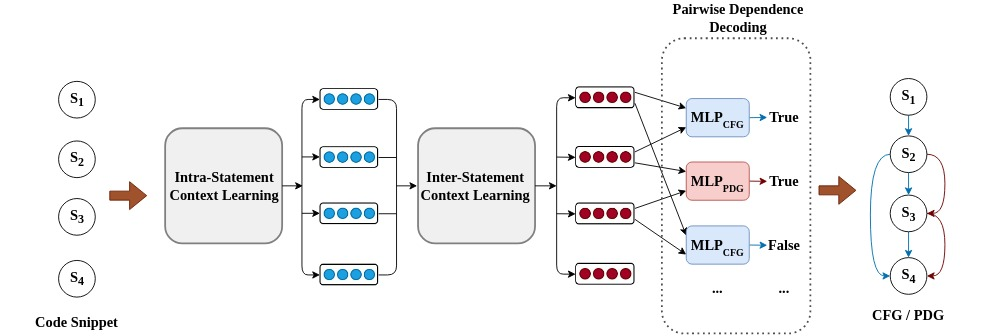
\includegraphics[width=\textwidth]{model-abstract.jpg}
    \caption{Preliminary Design for \tool Model.}
    \label{fig:model}
    \vspace{-12pt}
\end{center}
\end{figure*}

In Figure~\ref{fig:model}, we present a preliminary design of the general architecture of \tool model. Given that attention is the driver behind the now ubiquitous Transformers’~\cite{Vaswani-2017} success in efficiently learning representations for different entities in different contexts, we plan to make it the foundation of the context learning components in our model as well. Each is intended to learn different aspects of contextualization. For our preliminary empirical evaluation, we collected Java methods from the GitHub Java Corpus~\cite{githubCorpus2013} and generated their CFG/PDGs using Joern program analysis tool~\cite{joern-2014}. By employing a self-attention network for both intra-statement and inter-statement contextualization, we trained a bootstrap model on complete code. For testing, we treated each method individually and chose a consecutive portion within the method to predict the program dependencies, and compared them against the actual dependencies. Overall, our bootstrap model was able to predict CFG and PDG edges in Java programs with an F-score of 94.29\%.
